\documentclass[slovene]{book}
\usepackage{amsmath} 
\usepackage{amssymb} 
\usepackage{makeidx} 
\usepackage{graphicx} 

%Sk4 start
\usepackage{listings}
\usepackage{color}

\definecolor{dkgreen}{rgb}{0,0.6,0}
\definecolor{gray}{rgb}{0.5,0.5,0.5}
\definecolor{mauve}{rgb}{0.58,0,0.82}

\lstset{backgroundcolor = \color{lightgray},
	frame=tb,
  language=Java,
  aboveskip=3mm,
  belowskip=3mm,
  showstringspaces=false,
  columns=flexible,
  basicstyle={\small\ttfamily},
  numbers=none,
  numberstyle=\tiny\color{gray},
  keywordstyle=\color{blue},
  commentstyle=\color{dkgreen},
  stringstyle=\color{mauve},
  breaklines=true,
  breakatwhitespace=true,
  tabsize=3
}
%Sk4-end




\usepackage{epstopdf}
\usepackage{afterpage}
\usepackage[official]{eurosym}
\usepackage{tikz}
\usepackage{pgfplots} 
\usetikzlibrary{patterns}
\usetikzlibrary{pgfplots.groupplots} %Sk-3
\usepackage{placeins} %Sk-3
\usepackage{float}
\restylefloat{figure}


\usepackage{epstopdf}
\graphicspath{{img/}}

\usepackage{url}
\usepackage{babel}
\usepackage[T1]{fontenc}
\usepackage[utf8]{inputenc}

\usepackage{fancyhdr} %tole dodano za headerje, da jih lahko definiraš po želji (preostanek je v posameznem chapterju)

\usepackage{multicol} %Sk9

\usepackage{color}
\usepackage[normalem]{ulem}
% define red
\newcommand{\red}[1]{\textcolor{red}{#1}}

%\includeonly{chaptr2} %If you just want to process chaptr2.tex

%%%
% new commands
%%%

\newcommand{\eng}[1]{(angl.~\emph{#1})}

%%%
% definicija
%%%

\newtheorem{definicija}{Definicija}

%%%
% Zgled
%%%

\newtheorem{zgled}{Zgled}

%%%
% document
%%%

\begin{document}

\author{Uredil prof. dr. Miha Mraz}
\title{Analiza zmogljivosti oblačnih in strežniških storitev}
\date{Maj 2018}
\maketitle

\frontmatter
\tableofcontents
\chapter{Predgovor}

Pričujoče delo je razdeljeno v deset poglavij, ki predstavljajo analize zmogljivosti nekaterih tipičnih strežniških in oblačnih izvedenk računalniških sistemov in njihovih storitev. Avtorji posameznih poglavij so slušatelji predmeta \textit{Zanesljivost in zmogljivost računalniških sistemov}, ki se je v štud.letu 2017/2018 predaval na 1. stopnji univerzitetnega študija računalništva in informatike na Fakulteti za računalništvo in informatiko Univerze v Ljubljani. Vsem študentom se zahvaljujem za izkazani trud, ki so ga vložili v svoje prispevke.

\begin{flushright}
\textit{prof. dr. Miha Mraz, Ljubljana, v maju 2018}
\end{flushright}


\mainmatter

\chapter[Analiza zmogljivosti oblačnih storitev(Edi Čebokli, Rok Grmek, Tadej Škapin)]{Analiza zmogljivosti oblačnih storitev}

\pagestyle{fancy}
\fancyhf{}
\fancyhead[LE,RO]{\thepage}
\fancyhead[RE,LO]{\leftmark}

\huge Edi Čebokli, Rok Grmek, Tadej Škapin
\normalsize
\bigskip



\section{Opis problema}

Za izvedbo analize zmogljivosti oblačnih storitev smo si izbrali problem računanja števila \(\pi\) na oddaljenem strežniku.
Računamo ga na dva načina - po Leibnizovi \cite{3_leibniz} formuli:
\begin{equation}
    \frac{\pi}{4} = 1 + \frac{1}{3} + \frac{1}{5} + \frac{1}{7} +\frac{1}{9} + ...
\end{equation}
in po Bellardovi \cite{3_bellard} formuli:
\begin{equation}
    \pi = \frac{1}{2^6}\sum_{n=0}^{\infty}\frac{(-1)^n}{2^{10n}}(-\frac{2^5}{4n + 1} - \frac{1}{4n + 3} - \frac{2^8}{10n + 1} - \frac{2^6}{10n + 3} - \frac{2^2}{10n + 5} - \frac{2^2}{10n + 7} - \frac{1}{10n + 9}) .
\end{equation}
V obeh primerih je število \(\pi\) predstavljeno kot vsota neskončne vrste, seveda pa v praksi seštejemo le končno mnogo členov.
Pri tem se vsota večjega števila členov izraža v bolj natančnem izračunu, vendar pa s tem narašča časovna zahtevnost.
Želeli smo, da oba algoritma izračunata število \(\pi\) s podobno natančnostjo, to pa smo dosegli s seštevanjem prvih 24.473.399 členov Leibnizove formule in s seštevanjem le prvih dveh členov Bellardove formule.
V obeh primerih naš izračun odstopa od dejanske vrednosti števila \(\pi\) za približno \(10^{-7}\).

Oba algoritma smo implementirali v Python-u in C-ju, aplikacijo strežnika pa smo namestili pri treh različnih ponudnikih gostovanja (ti so podrobneje predstavljeni v razdelku \ref{3_ponudniki}).
V okviru analize zmogljivosti smo sistem obremenili tako, da smo z večkratnim pošiljanjem zahtev simulirali večje število odjemalcev (natančnejši opis bremena je v razdelku \ref{3_breme}).
To prikazuje tudi shema na sliki \ref{fig:3_shema_sistema}, kjer T1 označuje čas prenosa zahtevka od odjemalca do strežnika, T2 označuje čas potreben za izračun na strani strežnika, T3 pa čas prenosa rezultatov od strežnika do odjemalca.

\begin{figure}[H]
    \centering
    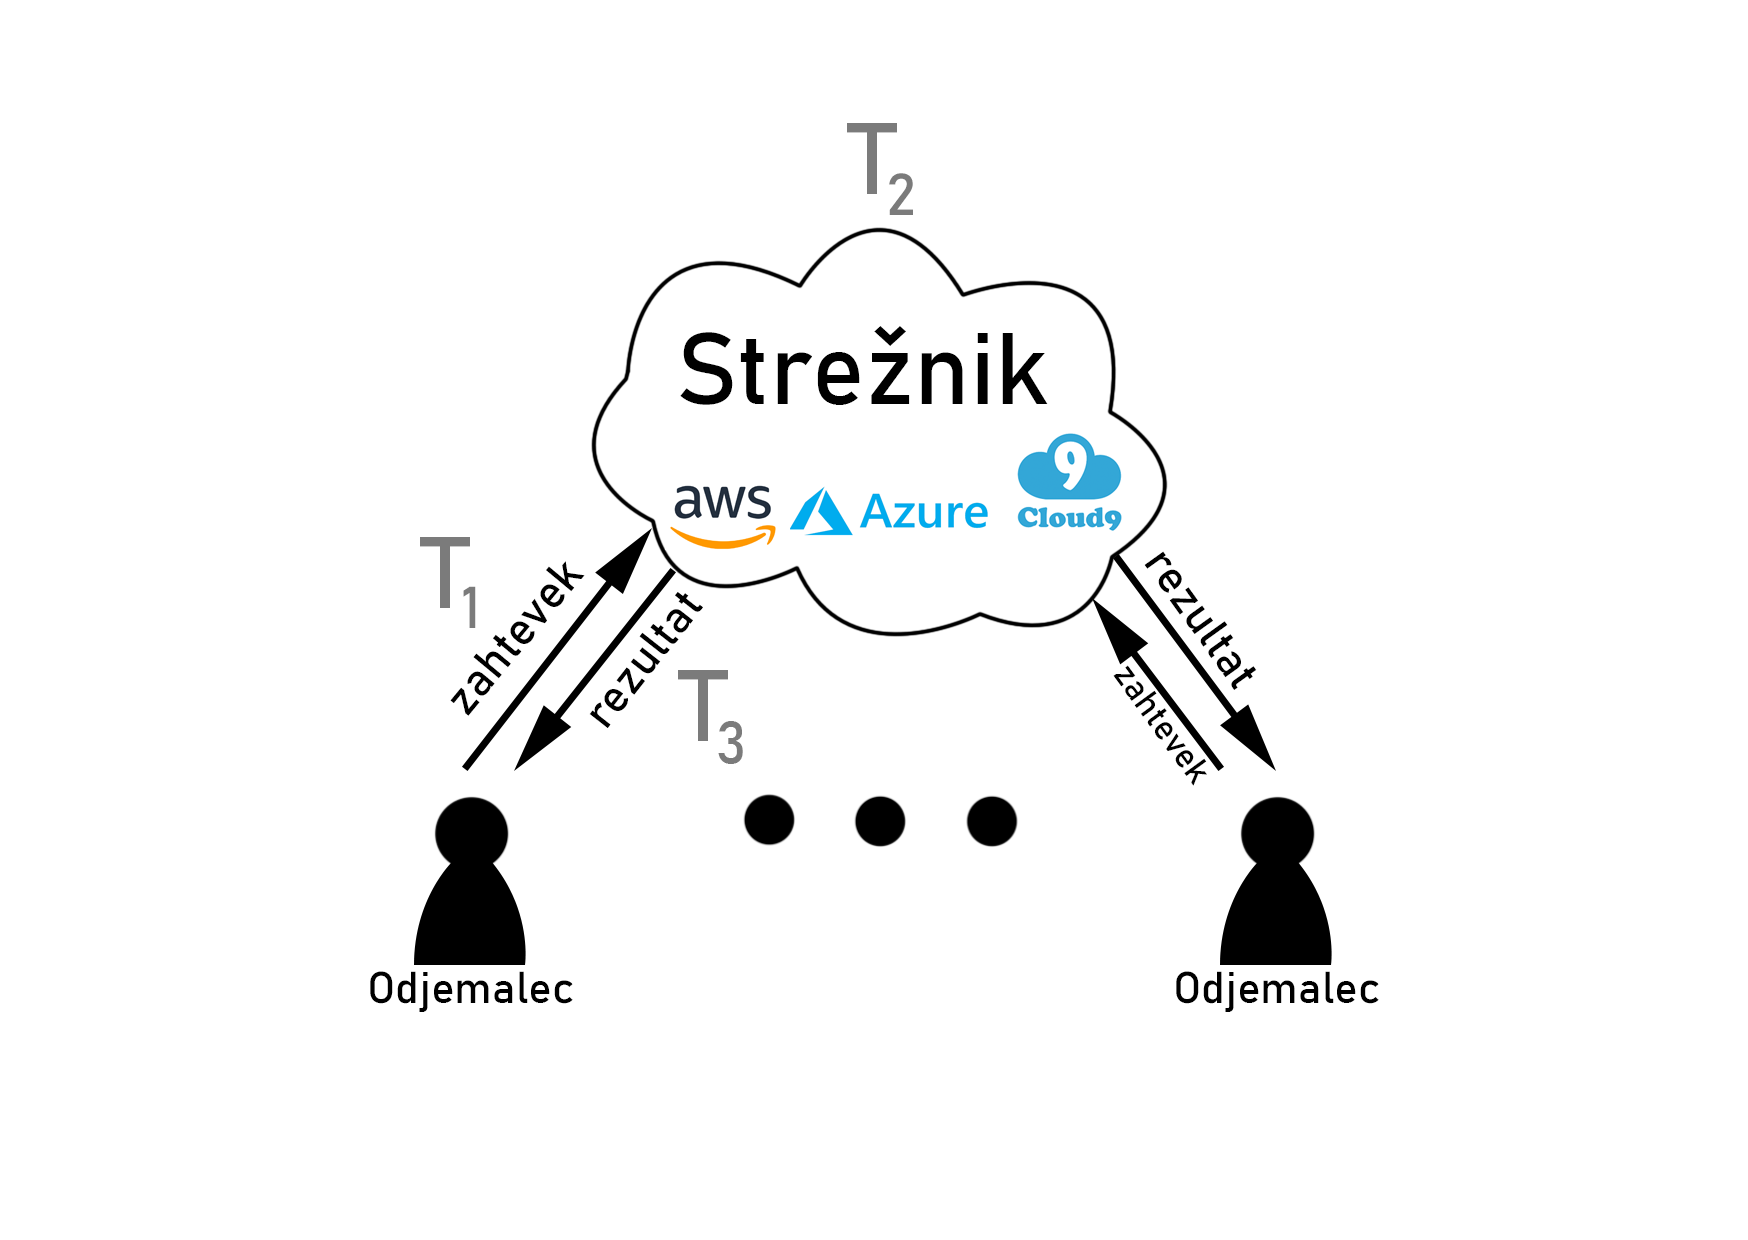
\includegraphics[scale=0.75]{3_shema.png}
    \caption{Shema pošiljanja zahtevkov na strežnik.}
    \label{fig:3_shema_sistema}
\end{figure}



\section{Pregled sorodnih virov}

Računanje števila \(\pi\) je numeričen problem, ki ga rešujemo s številnimi zaporednimi aritmetičnimi operacijami nad števili v plavajoči vejici (v dvojni natančnosti).
Zato smo že pred samim računanjem želeli preveriti, kako hitre so takšne operacije v primeru oblačnega računanja.
V članku ``A Performance Analysis of EC2 Cloud Computing Services for Scientific Computing'' \cite{3_ostermann2009performance} je analizirana zmogljivost računanja pri ponudniku gostovanja Amazon Web Services.
Med drugim so v članku predstavljeni tudi rezultati meritev, kjer je razvidno, kakšno število operacij (seštevanj/množenj v plavajoči vejici, v dvojni natančnosti) lahko strežnik izvede na sekundo.
Analizirani so sicer le plačljivi paketi, za te pa je pričakovana nekolika višja zmogljivost v primerjavi z brezplačnim paketom t2.micro, ki smo ga uporabili sami.
V povprečju so v analizi namerili približno 0.6 GOPS.
Glede na način izvajanja meritev, bomo lahko za računanje števila \(\pi\) po Leibnizovi formuli, implementirano v C-ju na koncu še sami izračunali povprečno število operacij na sekundo in ga primerjali z rezultatom iz prej omenjene analize zmogljivosti.



\section{Izbira tehnologij} \label{3_tehnologije}

Pri izbiri programskih jezikov smo izbrali Python in C, ki sta različna po načinu izvajanja programov.
Python je interpreterski jezik, ki hitreje analizira izvorno kodo, vendar počasneje izvaja program v primerjavi z eksekucijskim jezikom C.
Strežnik in odjemalec sta implementirana v Python-u, algoritma za računanje \(\pi\) pa v C-ju in Python-u.



\section{Ponudniki gostovanja} \label{3_ponudniki}

Aplikacijo strežnika za oddaljeno računanje števila \(\pi\) smo namestili pri treh različnih ponudnikih gostovanja - Amazon Web Services \cite{3_aws}, Microsoft Azure \cite{3_azure} in Cloud9 \cite{3_c9io}.
Za večino testov smo uporabili Amazon Web Services, v enem od testov pa so ponudniki neposredno primerjani med sabo.

Pri ponudniku Microsoft Azure smo izbrali paket A1 standard, pri AWS pa paket t2.micro.
To so paketi, ki jih lahko izberemo v brezplačni poskusni dobi uporabe storitve.
Specifikacija sistemov, ki jih ponujajo zgornji trije ponudniki, je navedena v tabeli \ref{3_tabela_specifikacij}.

\begin{table}[H]
    \centering
    \begin{tabular}{|p{1.4cm}|p{3.4cm}|p{1.4cm}|p{1.0cm}|p{0.9cm}|p{1.4cm}|}
        \hline
        Ponudnik  & CPE                    & Št. jeder  & RAM    & HDD   & Lokacija        \\
        \hline
        \hline
        AWS       & Intel Xeon E5-2676 v3  & 1          & 1GB    & 8GB   & Zahodna Evropa  \\
        \hline
        Azure     & Intel Xeon E5-2630 v3  & 1          & 1.5GB  & 30GB  & Južna Azija     \\
        \hline
        Cloud9    & Intel Xeon @2.50GHz    & 8          & 1GB    & 2GB   & ZDA             \\
        \hline
    \end{tabular}
    \caption{Tabela ponudnikov in njihovih specifikacij.}
    \label{3_tabela_specifikacij}
\end{table}



\section{Definicija bremena storitve} \label{3_breme}

Obremenjenost našega strežnika, ki ponuja oddaljeno računanje števila \(\pi\), je odvisna od izbrane metode računanja, od implementacije te metode in od intenzivnosti prejemanja zahtevkov za računanje.
Zato smo strežnik obremenili tako, da smo generirali večje število zaporednih zahtevkov za enega od načinov računanja, pri tem pa določili interval čakanja med dvema zahtevkoma.

Interval je v grobem lahko determinističen (točno določen), ali pa nedeterminističen (psevdo-naključno generiran in porazdeljen eksponentno).
Prva možnost omogoča lažjo analizo rezultatov zaradi konstantnega intervala, druga pa boljše opiše realno breme.

Pomembna je tudi delitev glede na to, kakšen je interval čakanja v primerjavi s časom računanja.
Velika razlika v obremenitvi sistema se namreč pojavi, če interval med dvema zahtevkoma zmanjšamo do te mere, da ta postane manjši od povprečnega časa računanja in zahtevki za računanje prihajajo pogosteje, kot jih lahko strežnik obdela.



\section{Definicija metrik in orodij za meritve}

Za posamezno računanje na oddaljenem strežniku dobimo kot rezultat poleg števila \(\pi\) tudi čas, ki ga je strežnik potreboval za računanje (T2), obenem pa merimo še celoten čas od pošiljanja zahtevka za računanje do prejetja rezultata (T1 + T2 + T3).
Pri eksperimentih nato opazujemo čas računanja na strežniku (T2) in čas, potreben za komunikacijo s strežnikom (T1 + T3).



\section{Rezultati meritev}

\subsection{Primerjava različnih načinov računanja}

\subsubsection{Opis eksperimenta}
    
Prve meritve smo opravili le pri ponudniku gostovanja AWS.
Za vsako od štirih različic izračuna smo strežniku 1 uro, iz enega klienta, na vsake 3 sekunde (deterministično) pošiljali zahtevke in ob tem merili čase.
S tem eksperimentom smo želeli preveriti delovanje sistema in primerjati štiri različne načine računanja med sabo.

\subsubsection{Hipoteza}

Pričakujemo lahko, da bodo časi računanja (T2) za vse 4 načine računanja skozi celoten čas testiranja približno konstantni.
Strežnik bo namreč vedno obdeloval le eno zahtevo na enkrat, ker nobeno računanje naj ne bi trajalo več kot 3 sekunde.

Računanje implementirano v Python-u bo najverjetneje trajalo dlje od tistega v C-ju (za isto metodo računanja), za vsako od implementacij pa bo Leibnizova metoda verjetno zahtevala več časa od Bellardove.
Kljub temu pa težko ocenimo, ali se bo iz časovnega vidika boljše odrezala Leibnizova metoda implementirana v C-ju ali Bellardova metoda implementirana v Python-u.

Čas komunikacije (T1 + T3) ni odvisen od načina računanja, zato sklepamo, da bo ta približno enak za vse štiri.
Ta čas bo najverjetneje približno konstanten tudi skozi celoten čas testiranja, saj ne pričakujemo večjih sprememb v zasedenosti omrežja med testiranjem.

\subsubsection{Okoliščine}

Meritve so bile opravljene v Ljubljani, s povezavo 100 Mbps / 10 Mbps.
Bile so opravljene med 18. in 19. uro v sredo 18. 4. 2018.
Vsaka meritev se je izvajala na svojem strežniku, vsi strežniki pa imajo identično konfiguracijo in lokacijo.

\subsubsection{Rezultati}

Čas računanja na strežniku (T2) v odvisnosti od časa testiranja je prikazan na sliki \ref{fig:3_rezultati1_T2}, celoten čas komunikacije (T1 + T3) spet v odvisnosti od časa testiranja pa je prikazan na sliki \ref{fig:3_rezultati1_T1T3}.

Hipoteza je bila očitno smiselna, iz rezultatov pa je vidno, da računanje po Bellardovi metodi zahteva manj časa v primerjavi z Leibnizovo metodo, ne glede na tehnologijo implementacije.

\begin{figure}[H]
    \begin{tikzpicture}
        \begin{axis}[
                        xlabel = Čas(min),
                        ylabel = T2(s),
                        legend pos = outer north east,
                    ]
            \addplot[smooth,blue] table[x index = {0}, y index = {3}] {3_rezultati1_leibniz_py.dat};
            \addlegendentry{$Leibnizova\ metoda - Python$}
            \addplot[smooth,red] table[x index = {0}, y index = {3}] {3_rezultati1_leibniz_c.dat};
            \addlegendentry{$Leibnizova\ metoda - C$}
            \addplot[smooth,gray] table[x index = {0}, y index = {3}] {3_rezultati1_bellard_py.dat};
            \addlegendentry{$Bellardova\ metoda - Python$}
            \addplot[smooth,green] table[x index = {0}, y index = {3}] {3_rezultati1_bellard_c.dat};
            \addlegendentry{$Bellardova\ metoda - C$}
        \end{axis}
    \end{tikzpicture}
    \caption{Čas računanja na strežniku v odvisnosti od časa testiranja.}
    \label{fig:3_rezultati1_T2}
\end{figure}

\begin{figure}[H]
    \begin{tikzpicture}
        \begin{axis}[
                        xlabel = Čas(min),
                        ylabel = T1 + T3(s),
                        legend pos = outer north east,
                    ]
            \addplot[smooth,blue] table[x index = {0}, y index = {4}] {3_rezultati1_leibniz_py.dat};
            \addlegendentry{$Leibnizova\ metoda - Python$}
            \addplot[smooth,red] table[x index = {0}, y index = {4}] {3_rezultati1_leibniz_c.dat};
            \addlegendentry{$Leibnizova\ metoda - C$}
            \addplot[smooth,gray] table[x index = {0}, y index = {4}] {3_rezultati1_bellard_py.dat};
            \addlegendentry{$Bellardova\ metoda - Python$}
            \addplot[smooth,green] table[x index = {0}, y index = {4}] {3_rezultati1_bellard_c.dat};
            \addlegendentry{$Bellardova\ metoda - C$}
        \end{axis}
    \end{tikzpicture}
    \caption{Celoten čas komunikacije v odvisnosti od časa testiranja.}
    \label{fig:3_rezultati1_T1T3}
\end{figure}



\subsection{Primerjava ponudnikov gostovanja}

\subsubsection{Opis eksperimenta}

Za ta eksperiment smo aplikacijo strežnika namestili pri treh različnih ponudnikih gostovanja (ti so predstavljeni v razdelku \ref{3_ponudniki}).
Zahtevke smo spet pošiljali 1 uro, na vsake 3 sekunde (deterministično), vendar tokrat do treh različnih strežnikov.
Na vsakem od strežnikov smo testirali le računanje z Leibnizovo metodo, implementirano v Python-u.

\subsubsection{Hipoteza}

Glede na specifikacije sistemov ponudnikov (tabela \ref{3_tabela_specifikacij}), pričakujemo podobne čase računanja (T2) za AWS in Azure, nekoliko krajše čase pa za Cloud9.

Časi komunikacije (T1 + T3) se bodo najverjetneje razlikovali zaradi različnih lokacij strežnikov.
Najkrajši čas pričakujemo za AWS, saj je strežnik lociran v Evropi, najdaljši čas pa bo verjetno potreben za dostop do strežnika v Južni Aziji, ki ga ponuja Azure.

\subsubsection{Okoliščine}

Meritve so bile opravljene v Ilirski Bistrici, s povezavo 20 Mbps / 5 Mbps.
Bile so opravljene med 14. in 15. uro v sredo 2. 5. 2018.

\subsubsection{Rezultati}

Čas računanja na strežniku (T2) v odvisnosti od časa testiranja je prikazan na sliki \ref{fig:3_rezultati2_T2}, celoten čas komunikacije (T1 + T3) spet v odvisnosti od časa testiranja pa je prikazan na sliki \ref{fig:3_rezultati2_T1T3}.

Rezultati se do neke mere ujemajo z dano hipotezo.
Nekoliko so nas presenetili časi računanja na strežniku, ki je bil nameščen pri ponudniku gostovanja Azure, saj so ti očitno precej višji od časov računanja na strežniku, nameščenem pri AWS.
Poleg tega, smo slabo predvideli tudi čase komunikacije s strežnikom, nameščenim pri Cloud9.
Ti so, za razliko od časov pri ostalih dveh ponudnikih, razpršeni na bistveno širšem intervalu in celo presegajo čase komunikacije s strežnikom, lociranim v Južni Aziji (Azure).

\begin{figure}[H]
    \begin{tikzpicture}
        \begin{axis}[
                        xlabel = Čas(min),
                        ylabel = T2(s),
                        legend pos = outer north east,
                    ]
            \addplot[smooth,blue] table[x index = {0}, y index = {3}] {3_rezultati2_aws.dat};
            \addlegendentry{$AWS$}
            \addplot[smooth,red] table[x index = {0}, y index = {3}] {3_rezultati2_azure.dat};
            \addlegendentry{$Azure$}
            \addplot[smooth,gray] table[x index = {0}, y index = {3}] {3_rezultati2_cloud9.dat};
            \addlegendentry{$Cloud9$}
        \end{axis}
    \end{tikzpicture}
    \caption{Čas računanja na strežniku v odvisnosti od časa testiranja.}
    \label{fig:3_rezultati2_T2}
\end{figure}

\begin{figure}[H]
    \begin{tikzpicture}
        \begin{axis}[
                        xlabel = Čas(min),
                        ylabel = T1 + T3(s),
                        legend pos = outer north east,
                    ]
            \addplot[smooth,blue] table[x index = {0}, y index = {4}] {3_rezultati2_aws.dat};
            \addlegendentry{$AWS$}
            \addplot[smooth,red] table[x index = {0}, y index = {4}] {3_rezultati2_azure.dat};
            \addlegendentry{$Azure$}
            \addplot[smooth,gray] table[x index = {0}, y index = {4}] {3_rezultati2_cloud9.dat};
            \addlegendentry{$Cloud9$}
        \end{axis}
    \end{tikzpicture}
    \caption{Celoten čas komunikacije v odvisnosti od časa testiranja.}
    \label{fig:3_rezultati2_T1T3}
\end{figure}



\subsection{Nedeterministično pošiljanje zahtevkov}

\subsubsection{Opis eksperimenta}
    
V prvih dveh eksperimentih smo zahtevke pošiljali deterministično, točno na vsake 3 sekunde.
Ker strežniki običajno niso obremenjeni na tak način, smo tokrat generirali zahtevke po Poissonovi porazdelitvi \cite{3_moskon_mraz_2012}, saj tak model boljše ponazori običajen promet.
Časovni interval med dvema zahtevkoma je v takem primeru porazdeljen eksponentno s parametrom \(\lambda\), pričakovana vrednost intervala pa je enaka \(\frac{1}{\lambda}\).
V našem primeru smo želeli v povprečju ohraniti 3 sekundni interval, zato smo uporabili parameter porazdelive ali intenzivnosti porajanja zahtev \(\lambda=\frac{1}{3}\) zahteve na sekundo.
Eksperiment je tudi tokrat trajal 1 uro, meritve pa smo opravili le pri ponudniku gostovanja AWS in sicer za računanje po Leibnizovi metodi, implementirano v Python-u.

\subsubsection{Hipoteza}

Čas računanja (T2) bo v najboljšem primeru enak tistemu iz eksperimenta z determinističnim intervalom pošiljanja zahtevkov, lahko pa pričakujemo, da se bodo nekateri zahtevki obdelovali nekoliko dlje.
Zaradi naključnosti modela, se bo namreč zelo verjetno zgodilo to, da bo nek zahtevek poslan še preden bo prejšnji obdelan, kar pa bo prineslo daljši čas računanja.

Sprememba modela za generiranje zahtevkov najverjetneje ne bo vplivala na čas komunikacije (T1 + T3), zato predvidevamo, da bo ta čas ostal nespremenjen.

\subsubsection{Okoliščine}

Meritve so bile opravljene v Ilirski Bistrici, s povezavo 20 Mbps / 5 Mbps.
Bile so opravljene med 11. in 12. uro v ponedeljek 30. 4. 2018.

\subsubsection{Rezultati}

Čas računanja na strežniku (T2) v odvisnosti od časa testiranja je prikazan na sliki \ref{fig:3_rezultati3_T2}, celoten čas komunikacije (T1 + T3) spet v odvisnosti od časa testiranja pa je prikazan na sliki \ref{fig:3_rezultati3_T1T3}.
Ti rezultati popolnoma potrjujejo dano hipotezo.

\begin{figure}[H]
    \begin{tikzpicture}
        \begin{axis}[
                        xlabel = Čas(min),
                        ylabel = T2(s),
                        legend pos = outer north east,
                    ]
            \addplot[smooth,blue] table[x index = {0}, y index = {3}] {3_rezultati3.dat};
        \end{axis}
    \end{tikzpicture}
    \caption{Čas računanja na strežniku v odvisnosti od časa testiranja.}
    \label{fig:3_rezultati3_T2}
\end{figure}

\begin{figure}[H]
    \begin{tikzpicture}
        \begin{axis}[
                        xlabel = Čas(min),
                        ylabel = T1 + T3(s),
                        legend pos = outer north east,
                    ]
            \addplot[smooth,blue] table[x index = {0}, y index = {4}] {3_rezultati3.dat};
        \end{axis}
    \end{tikzpicture}
    \caption{Celoten čas komunikacije v odvisnosti od časa testiranja.}
    \label{fig:3_rezultati3_T1T3}
\end{figure}



\subsection{Ogrevanje sistema (postopno večanje obremenitve)}

\subsubsection{Opis eksperimenta}

V predhodnih eksperimentih nismo nikoli pošiljali zahtevkov bolj pogosto, kot jih je strežnik lahko obdelal (v povprečju), zato smo pripravili eksperiment, kjer postopoma višamo frekvenco pošiljanja zahtevkov.
Najprej smo 5 minut pošiljali zahtevke na vsake 3 sekunde, naslednjih 5 minut na 2 sekundi, nato 5 minut vsako sekundo, zadnjih 5 minut pa vsake 0,5 sekunde (vsi intervali čakanja so bili generirani deterministično).
Računali smo z Leibnizovo metodo, implementirano v Pythonu, strežnik pa smo namestili pri ponudniku gostovanja AWS.

\subsubsection{Hipoteza}

Prvih 10 minut lahko pričakujemo konstanten čas računanja (T2), saj še vedno pošiljamo zahtevke dovolj počasi.
Interval med dvema zahtevkoma je namreč v tem delu testiranja najprej enak 3 in nato 2 sekundi, kar je več od povprečnega časa trajanja enega izračuna.
Naslednjih 5 minut bo čas računanja najverjetneje začel linearno naraščati, saj se program izvaja več kot 1 sekundo, kar pomeni, da bodo novi zahtevki prihajali hitreje kot se lahko obdelajo in bo hkrati v obdelavi vedno več zahtevkov.
Enako velja za naslednjih 5 minut, vendar pričakujemo še hitrejše naraščanje časa računanja.

Čas komunikacije (T1 + T3) bo najverjetneje konstanten skozi vse 4 faze, saj ta eksperiment predstavlja večjo obremenitev predvsem za strežnik, ne pa tudi za omrežje.
Zahtevke namreč pošiljamo kvečjemu 2-krat na sekundo, paketi pa so ranga velikosti nekaj KB.

\subsubsection{Okoliščine}

Meritve so bile opravljene v Ilirski Bistrici, s povezavo 20 Mbps / 5 Mbps.
Bile so opravljene med 14. in 15. uro v ponedeljek 30. 4. 2018.

\subsubsection{Rezultati}

Čas računanja na strežniku (T2) v odvisnosti od časa testiranja je prikazan na sliki \ref{fig:3_rezultati4_T2}, celoten čas komunikacije (T1 + T3) spet v odvisnosti od časa testiranja pa je prikazan na sliki \ref{fig:3_rezultati4_T1T3}.

Pri postavljanju hipoteze smo tokrat naredili napako.
Skozi prvi dve fazi so časi računanja res konstantni in nato nekaj časa naraščajo, vendar se malo pred koncem tretje faze naraščanje upočasni, kot bi se časi približevali neki zgornji meji, nato pa ti časi celo padajo.
Približevanje zgornji meji je smiselno, saj strežnik ne more hkrati obdelovati poljubnega števila zahtevkov (zaradi končnega pomnilnika) in zato ta v neki točki začne spuščati zahtevke (od strežnika smo namreč prejeli le 692 odgovorov za 1150 poslanih zahtevkov).
Padanje časov je najverjetneje povezano s koncem eksperimenta.
Tisti zadnji zahtevki se (za razliko od predhodnih) obdelujejo še po koncu ekpserimenta, takrat pa novi zahtevki ne prihajajo več na strežnik.
Nekaj časa na koncu se torej manjša število zahtevkov, ki so hkrati v obdelavi, to pa pomeni krajše čase računanja.

Tudi časi komunikacije se nekoliko razlikujejo od pričakovanih, vendar to odstopanje povezujemo z napako pri merjenju časa računanja (T2) v primeru, ko strežnik obdeluje veliko število zahtevkov hkrati.
Lahko se zgodi, da zaradi zelo velikega števila niti, ki obdelujejo posamezne zahtevke, glavna nit, ki sprejema zahtevke in meri čas računanja, nekaj časa ne pride na vrsto in posledično zamudi pri beleženju časa, ko je zahtevek prišel do strežnika.
Ta napaka se odraža kot nekaj sekundni pribitek času komunikacije in enako dolg odbitek času računanja, žal pa je odvisna od operacijskega sistema, ki razvršča niti in je ne moremo odpraviti.

\begin{figure}[H]
    \begin{tikzpicture}
        \begin{axis}[
                        xlabel = Čas(min),
                        ylabel = T2(s),
                        legend pos = outer north east,
                    ]
            \addplot[smooth,blue] table[x index = {0}, y index = {3}] {3_rezultati4.dat};
        \end{axis}
    \end{tikzpicture}
    \caption{Čas računanja na strežniku v odvisnosti od časa testiranja.}
    \label{fig:3_rezultati4_T2}
\end{figure}

\begin{figure}[H]
    \begin{tikzpicture}
        \begin{axis}[
                        xlabel = Čas(min),
                        ylabel = T1+T3(s),
                        legend pos = outer north east,
                    ]
            \addplot[smooth,blue] table[x index = {0}, y index = {4}] {3_rezultati4.dat};
        \end{axis}
    \end{tikzpicture}
    \caption{Celoten čas komunikacije v odvisnosti od časa testiranja.}
    \label{fig:3_rezultati4_T1T3}
\end{figure}



\subsection{Konstantna visoka obremenitev} \label{3_konst_vis_obr}

\subsubsection{Opis eksperimenta}

Pri prejšnjem eksperimentu so nas rezultati rahlo presenetili, zato smo želeli našo interpretacijo rezultatov preveriti še z dodatnim eksperimentom.
V ta namen smo tokrat izvedli meritve le za tretjo fazo prejšnjega eksperimenta (deterministično pošiljanje zahtevkov na vsako sekundo), vendar smo eksperiment izvajali več časa - 1 uro.

\subsubsection{Hipoteza}

Pričakujemo, da bodo časi računanja (T2) najprej naraščali dokler ne dosežejo zgornje meje, nato bodo večji del testiranja ti časi približno konstantni, pred koncem pa se bodo časi spet zmanjšali.

Čas komunikacije (T1 + T3) bo najverjetneje spet višji kot bi bilo smiselno, vendar bo to zaradi napake merjenja časov, omenjene pri prejšnjem eksperimentu.
Če so višji izmerjeni časi komunikacije res posledica napake, potem bodo ti časi tudi nekoliko korelirani s časi računanja.
Časi računanja namreč dobro kažejo na obremenjenost sistema z velikim številom hkrati aktivnih niti, velikost napake pa je odvisna ravno od števila niti, ki si z glavno nitjo delijo računske vire.

\subsubsection{Okoliščine}

Meritve so bile opravljene v Ilirski Bistrici, s povezavo 20 Mbps / 5 Mbps.
Bile so opravljene med 15. in 16. uro v ponedeljek 30. 4. 2018.

\subsubsection{Rezultati}

Čas računanja na strežniku (T2) v odvisnosti od časa testiranja je prikazan na sliki \ref{fig:3_rezultati5_T2}, celoten čas komunikacije (T1 + T3) spet v odvisnosti od časa testiranja pa je prikazan na sliki \ref{fig:3_rezultati5_T1T3}.

Rezultati se ujemajo z dano hipotezo, to pa potrjuje tudi celotno interpretacijo rezultatov iz prejšnjega eksperimenta.

Zanimivo je še pogledati število zahtevkov, ki so bili na strežniku spuščeni.
Od 3600 poslanih zahtevkov, smo odgovor dobili le za 2049 zahtevkov.
V eni uri je strežnik torej 2049-krat uspešno izračunal število \(\pi\), kar pomeni, da je za posamezen izračun efektivno potreboval le 1,76 s (\(\frac{3600 s}{2049}\)), ta čas je pa zelo podoben času, ki ga tak strežnik potrebuje za en izračun, ko sploh ni preobremenjen.
Iz tega sledi, da strežnik v primeru preobremenitve spusti praktično najmanjše možno število zahtevkov.
Če bi želeli spuščanje zahtevkov popolnoma preprečiti, bi te lahko generirali kvečjemu na vsake 1,76 s (interval je torej potrebno prilagoditi času, ki ga strežnik potrebuje za en izračun).

\begin{figure}[H]
    \begin{tikzpicture}
        \begin{axis}[
                        xlabel = Čas(min),
                        ylabel = T2(s),
                        legend pos = outer north east,
                    ]
            \addplot[smooth,blue] table[x index = {0}, y index = {3}] {3_rezultati5.dat};
        \end{axis}
    \end{tikzpicture}
    \caption{Čas računanja na strežniku v odvisnosti od časa testiranja.}
    \label{fig:3_rezultati5_T2}
\end{figure}

\begin{figure}[H]
    \begin{tikzpicture}
        \begin{axis}[
                        xlabel = Čas(min),
                        ylabel = T1 + T3(s),
                        legend pos = outer north east,
                    ]
            \addplot[smooth,blue] table[x index = {0}, y index = {4}] {3_rezultati5.dat};
        \end{axis}
    \end{tikzpicture}
    \caption{Celoten čas komunikacije v odvisnosti od časa testiranja.}
    \label{fig:3_rezultati5_T1T3}
\end{figure}



\subsection{Primerjava različno intenzivnih preobremenitev}

\subsubsection{Opis eksperimenta}

Pri prejšnjem eksperimentu smo zahtevke pošiljali pogosteje kot jih lahko strežnik obdela in opazili, da se v neki točki časi računanja ustalijo.
To se zgodi, ko je dosežena zgornja meja za število zahtevkov, ki se lahko hkrati obdelujejo (tisti zahtevki, ki bi to mejo presegli pa so izpuščeni in nanje ne dobimo odgovora).
S tem eksperimentom bi radi preverili, do kakšne spremembe pride pri časih računanja, če zahtevke pošiljamo nekoliko pogosteje ali pa nekoliko redkeje (vendar še vedno bolj pogosto, kot jih lahko strežnik obdela).
Zato smo tokrat 20 minut deterministično pošiljali zahtevke, na vsake 0,8 s, na vsako sekundo ter na vsake 1,2 s do strežnika, nameščenega pri ponudniku AWS. Eksperimenti so potekali istočasno, vsak na svoji instanci. Vse instance so identične.

\subsubsection{Hipoteza}

Čas računanja je v našem primeru odvisen od števila zahtevkov, ki se hkrati obdelujejo, zato pričakujemo, da bodo časi računanja naraščali hitreje v primeru, kjer pogosteje pošiljamo zahtevke in obratno.
Poleg tega, lahko pričakujemo, da se bodo v vseh treh primerih časi ustalili pri približno enaki vrednosti, saj bo meja, pri kateri strežnik spušča zahtevke enaka v vseh treh primerih, ne glede na to, kako pogosto pošiljamo zahtevke.

Pri časih komunikacije ne pričakujemo večjih razlik, saj noben od treh primerov pošiljanja zahtevkov ne predstavlja resnejše obremenitve za omrežje. Po drugi strani pa v vseh treh primerih vseeno pričakujemo prisotnost že omenjene napake pri merjenju časov, saj bo sistem obremenjen s precej visokim številom niti.

\subsubsection{Okoliščine}

Meritve so bile opravljene v Sežani, s povezavo 10 Mbps / 10 Mbps.
Bile so opravljene med 7. in 8. uro v soboto 19. 5. 2018.

\subsubsection{Rezultati}

Čas računanja na strežniku (T2) v odvisnosti od časa testiranja je prikazan na sliki \ref{fig:3_rezultati6_T2}, celoten čas komunikacije (T1 + T3) spet v odvisnosti od časa testiranja pa je prikazan na sliki \ref{fig:3_rezultati6_T1T3}.

Hipoteza se je izkazala za pravilno, saj časi računanja najprej naraščajo intervalu primerno, nato pa se v vseh treh primerih ustalijo na približno 500 s.
Tudi časi komunikacije ustrezajo hipotezi, vključno z omenjeno napako, ki je še posebej vidna v primeru 1,2 s intervala.

\begin{figure}[H]
    \begin{tikzpicture}
        \begin{axis}[
                        xlabel = Čas(min),
                        ylabel = T2(s),
                        legend pos = outer north east,
                    ]
            \addplot[smooth,blue] table[x index = {0}, y index = {3}] {3_rezultati6_08.dat};
            \addlegendentry{$0,8 s$}
            \addplot[smooth,red] table[x index = {0}, y index = {3}] {3_rezultati6_10.dat};
            \addlegendentry{$1,0 s$}
            \addplot[smooth,gray] table[x index = {0}, y index = {3}] {3_rezultati6_12.dat};
            \addlegendentry{$1,2 s$}
        \end{axis}
    \end{tikzpicture}
    \caption{Čas računanja na strežniku v odvisnosti od časa testiranja.}
    \label{fig:3_rezultati6_T2}
\end{figure}

\begin{figure}[H]
    \begin{tikzpicture}
        \begin{axis}[
                        xlabel = Čas(min),
                        ylabel = T1 + T3(s),
                        legend pos = outer north east,
                    ]
            \addplot[smooth,blue] table[x index = {0}, y index = {4}] {3_rezultati6_08.dat};
            \addlegendentry{$0,8 s$}
            \addplot[smooth,red] table[x index = {0}, y index = {4}] {3_rezultati6_10.dat};
            \addlegendentry{$1,0 s$}
            \addplot[smooth,gray] table[x index = {0}, y index = {4}] {3_rezultati6_12.dat};
            \addlegendentry{$1,2 s$}
        \end{axis}
    \end{tikzpicture}
    \caption{Celoten čas komunikacije v odvisnosti od časa testiranja.}
    \label{fig:3_rezultati6_T1T3}
\end{figure}



\subsection{Eksperimentalno določanje meje preobremenitve}

\subsubsection{Opis eksperimenta}

V enem od prejšnjih eksperimentov (razdelek \ref{3_konst_vis_obr}) je že bilo govora o največji možni obremenitvi strežnika, pri kateri se zahtevki pravočasno obdelujejo in se novi zahtevki ne kopičijo v vrsti.
Predvideli smo, da je interval pošiljanja potrebno prilagoditi povprečnemu času računanja posameznega zahtevka, s tem eksperimentom pa bi to želeli še dodatno preveriti.
V našem primeru je za strežnik, nameščen pri ponudniku gostovanja AWS ta čas enak približno 1,76 s.
Zato smo tokrat za gostovanje spet uporabili ponudnika AWS, zahtevke pa smo 20 minut pošiljali nedeterministično z intervali 1,70 s, 1,75 s ter 1,80 s.  Eksperimenti so potekali istočasno, vsak na svoji instanci. Vse instance so identične.

\subsubsection{Hipoteza}

Najverjetneje bodo časi računanja v obeh primerih, kjer je interval generiranja zahtevkov nižji od povprečnega časa računanja nekoliko naraščali skozi čas, v primeru višjega intervala pa pričakujemo, da bo čas računanja približno konstanten.
Seveda ne smemo pozabiti, da se tokrat zahtevki generirajo nedeterministično, kar pomeni, da bo pri vseh treh primerih prisotno tudi nekakšno nihanje v časih računanja - zgornje trditve se torej nanašajo bolj na trend, kot pa na dejansko gibanje vrednosti skozi čas.

Pri časih komunikacije v tem eksperimentu ne pričakujemo nobenih večjih posebnosti.

\subsubsection{Okoliščine}

Meritve so bile opravljene v Sežani, s povezavo 10 Mbps / 10 Mbps.
Bile so opravljene med 13. in 14. uro v soboto 19. 5. 2018.

\subsubsection{Rezultati}

Čas računanja na strežniku (T2) v odvisnosti od časa testiranja je prikazan na sliki \ref{fig:3_rezultati7_T2}, celoten čas komunikacije (T1 + T3) spet v odvisnosti od časa testiranja pa je prikazan na sliki \ref{fig:3_rezultati7_T1T3}.

Na prvi pogled izgledajo časi računanja v vseh treh primerih precej podobno, vendar lahko opazimo, da se v primeru 1,80 s intervala časi računanja po naraščanju vedno vrnejo do običajnega nivoja, v ostalih dveh primerih pa časi postopoma naraščajo intervalu primerno in s tem kažejo na predpostavljeno preobremenitev.
S časi komunikacije v tem eksperimentu res ni bilo posebnosti.
Izkaže se, da ti sploh niso korelirani z intervalom pošiljanja zahtevkov, kar je tudi smiselno za tako majhne razlike v obremenitvi omrežja.


\begin{figure}[H]
    \begin{tikzpicture}
        \begin{axis}[
                        xlabel = Čas(min),
                        ylabel = T2(s),
                        legend pos = outer north east,
                    ]
            \addplot[smooth,blue] table[x index = {0}, y index = {3}] {3_rezultati7_170.dat};
            \addlegendentry{$1,70 s$}
            \addplot[smooth,red] table[x index = {0}, y index = {3}] {3_rezultati7_175.dat};
            \addlegendentry{$1,75 s$}
            \addplot[smooth,gray] table[x index = {0}, y index = {3}] {3_rezultati7_180.dat};
            \addlegendentry{$1,80 s$}
        \end{axis}
    \end{tikzpicture}
    \caption{Čas računanja na strežniku v odvisnosti od časa testiranja.}
    \label{fig:3_rezultati7_T2}
\end{figure}

\begin{figure}[H]
    \begin{tikzpicture}
        \begin{axis}[
                        xlabel = Čas(min),
                        ylabel = T1 + T3(s),
                        legend pos = outer north east,
                    ]
            \addplot[smooth,blue] table[x index = {0}, y index = {4}] {3_rezultati7_170.dat};
            \addlegendentry{$1,70 s$}
            \addplot[smooth,red] table[x index = {0}, y index = {4}] {3_rezultati7_175.dat};
            \addlegendentry{$1,75 s$}
            \addplot[smooth,gray] table[x index = {0}, y index = {4}] {3_rezultati7_180.dat};
            \addlegendentry{$1,80 s$}
        \end{axis}
    \end{tikzpicture}
    \caption{Celoten čas komunikacije v odvisnosti od časa testiranja.}
    \label{fig:3_rezultati7_T1T3}
\end{figure}



\subsection{24-urni eksperiment}

\subsubsection{Opis eksperimenta}

S prejšnjim eksperimentom smo potrdili, da mejni interval generiranja zahtevkov, preden sistem preobremenimo, leži nekje med 1,75 s ter 1,80 s (za ponudnika gostovanja AWS).
Kot zadnji eksperiment pa smo želeli pripraviti še testiranje, kjer sistem obremenimo na približno dve tretjini mejne obremenitve, vendar takšno obremenitev vzdržujemo celih 24 ur.
Zahtevke smo torej pošiljali 24 ur do strežnika, nameščenega pri ponudniku gostovanja AWS, nedeterministično z intervalom 2,65 s.

\subsubsection{Hipoteza}

Ta eksperiment simulira promet, pri katerem uporabniki občiajno že opazijo, da sistem deluje rahlo počasneje kot sicer.
Pričakujemo torej nekoliko višje čase računanja (v primerjavi s časom, ki je potreben za obdelavo enega samega zahtevka).

Pri časih komunikacije tudi tokrat ne pričakujemo večjih posebnosti. Pozorni bomo lahko na razlike skozi različne ure dneva, vendar nismo prepričani, če bodo te razlike dovolj očitne.

\subsubsection{Okoliščine}

Meritve so bile opravljene v Sežani, s povezavo 10 Mbps / 10 Mbps.
Bile so opravljene med 14. uro v soboto 19. 5. 2018 in 14. uro v nedeljo 20. 5. 2018.

\subsubsection{Rezultati}

Čas računanja na strežniku (T2) v odvisnosti od časa testiranja je prikazan na sliki \ref{fig:3_rezultati8_T2}, celoten čas komunikacije (T1 + T3) spet v odvisnosti od časa testiranja pa je prikazan na sliki \ref{fig:3_rezultati8_T1T3}.

Rezultati v celoti potrjujejo hipotezo.
V najslabšem primeru je računanje trajalo skoraj 40 s (sicer pa za obdelavo enega samega zahtevka v povprečju preteče približno 1,76 s).
Iz časov komunikacije žal ne razberemo odvisnosti od ure dneva.

\begin{figure}[H]
    \begin{tikzpicture}
        \begin{axis}[
                        xlabel = Čas(h),
                        ylabel = T2(s),
                        legend pos = outer north east,
                    ]
            \addplot[smooth,blue] table[x index = {0}, y index = {3}] {3_rezultati8.dat};
        \end{axis}
    \end{tikzpicture}
    \caption{Čas računanja na strežniku v odvisnosti od časa testiranja.}
    \label{fig:3_rezultati8_T2}
\end{figure}

\begin{figure}[H]
    \begin{tikzpicture}
        \begin{axis}[
                        xlabel = Čas(h),
                        ylabel = T1 + T3(s),
                        legend pos = outer north east,
                    ]
            \addplot[smooth,blue] table[x index = {0}, y index = {4}] {3_rezultati8.dat};
        \end{axis}
    \end{tikzpicture}
    \caption{Celoten čas komunikacije v odvisnosti od časa testiranja.}
    \label{fig:3_rezultati8_T1T3}
\end{figure}



\section{Zaključek}

Z zgornjimi eksperimenti smo ovrednotili časovno zahtevnost štirih različnih načinov računanja števila \(\pi\) in zmogljivost strežnikov pri treh različnih ponudnikih gostovanja.
Iz rezultatov lahko razberemo, da je Bellardova metoda konstantno hitrejša od Leibnizove ne glede na implementacijo.
Prav tako lahko opazimo, da je računanje pri ponudniku Cloud9 najhitrejše, pri Azure najpočasnejše, AWS pa pade nekje vmes.
Drugačno razporeditev vidimo pri času komunikacije, kjer je pri ponudniku AWS najkrajši, zaradi nam ugodne lokacije strežnikov.
Azure in Cloud9 imata podoben čas komunikacije, vendar ima slednji veliko večjo varianco.

S stopnjevanim determinističnim pošiljanjem zahtevkov smo prišli do ugotovitve, da strežnik pri preveliki obremenitvi začne spuščati zahtevke. Na podlagi te ugotovitve, smo z dodatnim testom določili zgornjo mejo obremenitve (1,76 s), pri kateri strežnik še obdela vse poslane zahtevke (ne glede na čas testiranja).
V eksperimentu 1.6.6 smo opazovali tudi kako različni intervali pošiljanja zahtevkov vplivajo na hitrost polnjenja vrste, pri tem pa smo tudi določili zgornjo mejo časa izračuna posameznega zahtevka (v primeru maksimalnega števila zahtevkov v hkratni obdelavi).
Opazimo tudi, da proti koncu testiranja strežnik potrebuje vse manj časa za obdelavo posameznega zahtevka, saj se po zadnjem poslanem zahtevku, hkrati obdeluje vedno manjše število zahtevkov.
To potrdimo še z dodatnim eksperimentom, kjer zahtevke eno uro deterministično pošiljamo vsako sekundo.

Ko smo določili zgornjo mejo frekvence determinističnega pošiljanja zahtevkov, smo strežnik preizkusili tudi na način ki simulira realno okolje.
Zahtevke smo večkrat nedeterministično pošiljali z različnimi frekvencami, blizu predvidene meje preobremenitve.
Opazimo, da se zahtevki na strežniku počasi kopičijo in včasih nastanejo daljše čakalne vrste, kljub temu pa v primeru, ko pošiljamo z nekoliko manjšo frekvenco od predvidene meje preobremenitve, ne izgubimo nobenega zahtevka.
Za konec na strežnik nedeterministično pošiljamo zahtevke pri \(\frac{2}{3}\) sposobnosti delovanja strežnika, saj je to meja pri kateri uporabnik občuti zakasnitve.
Čas obdelovanja zahtev je v tem primeru podoben kot v prvem eksperimentu, kjer strežnik ni bil tako intenzivno obremenjen, le da občasno pride do nekoliko večjih časov računanja.

V primerjavi z meritvami v članku ``A Performance Analysis of EC2 Cloud Computing Services for Scientific Computing'' \cite{3_ostermann2009performance}, kjer so namereli 0.6 GOPS je naš rezultat z brezplačnim paketom t2.micro približno 0.42 GOPS.
To smo izračunali s pomočjo Leibnizove metode implementirane v c-ju.
Celoten čas izračuna je približno 0,12 s, za izračun je pa potrebnih približno 25 milijonov seštevanj in deljenj.
V enem izračunu se torej zgodi približno 50 milijonov operacij, opravimo pa lahko 8,3 izračunov na sekundo kar pomeni da dosežemo 0,416 GOPS.
Teoretična maksimalna zmogljivost procesorja je 4,4 GOPS \cite{3_ostermann2009performance}, ponudnik pa nam da na razpolago 10 odstotkov tega \cite{3_10odstotkov}, torej 0,44 GOPS.
To pomeni, da je bilo v času našega testiranja izkoriščenih 94,5\% računske moči.


 
%\include{poglavjeN} 

\backmatter
%\include{glossary}
%\include{notat}
\bibliographystyle{ieeetr} %The style you want to use for references.
\bibliography{mro} %The files containing all the articles and books you ever referenced.
\printindex %Make an index AUTOMATICALLY

\end{document} 
